\chapter[\texttt C\'alculo del factor de correccion para $\Phi_f$]{Factor de correcci\'on para la eficiencia cu\'antica de fluorescencia}{}\label{apendicitis} %\vspace{-30pt}

%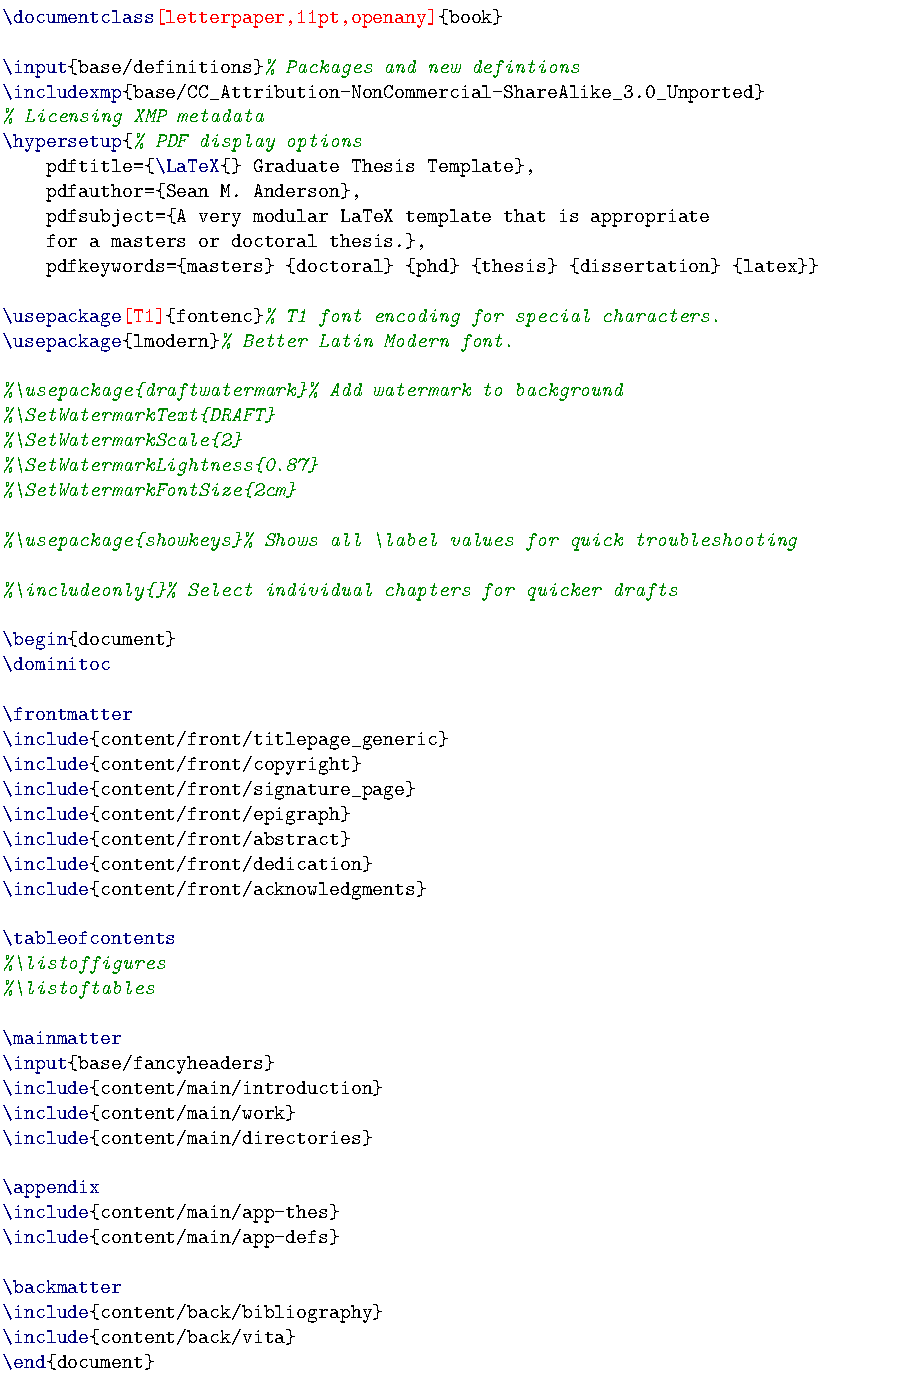
\includegraphics[height=0.90\textheight]{appendices/app-thesis}
%\chapter{Ap\'endices}
%\section{C\'alculo del factor de correccion del PMT}\label{apendicitis} 

En la figura \ref{kk} se muestra la curva de sensibilidad de respuesta contra longitud de onda que tiene el PMT modelo R7400U-01. 

Cuando la fluorescencia de la muestra de inter\'es y de la referencia (Rodamina 6G) tienen longitudes de onda similares, el PMT responder\'a de la misma manera en ambas muestras; sin embargo, si la muestra y la referencia emiten en diferentes longitudes de onda es necesario considerar un factor de correcci\'on.

Inicialmente se consider\'o que para la Rodamina 6G, la longitud de onda en la que se presenta la m\'axima emisi\'on es de 600 $nm$. El factor de correcci\'on se determin\'o calculando la raz\'on entre el valor de sensibilidad a 600 $nm$ y el valor de sensibilidad a la longitud de onda de mayor emisi\'on de la muestra de inter\'es. Finalmente para obtener el valor m\'as preciso de $\Phi_f$ se multiplic\'o el factor de correcci\'on por el valor de $\Phi_f$ que se obtiene sin tomar en cuenta la curva de sensibilidad del PMT. 

Por ejemplo, para el caso de la mol\'ecula octopolar en soluci\'on de THF, la cual emit\'ia en azul (450 $nm$), el factor de correcci\'on fue 0.6 o bien $30/50$ que son los valores de sensibilidad a 600 y 450 $nm$ respectivamente. Este valor se multiplic\'o por $\Phi_{fPromedio}=0.44$ para obtener $\Phi_f=0.26$ como se indic\'o en la tabla \ref{tablita}.

\begin{figure}[h]
\centering
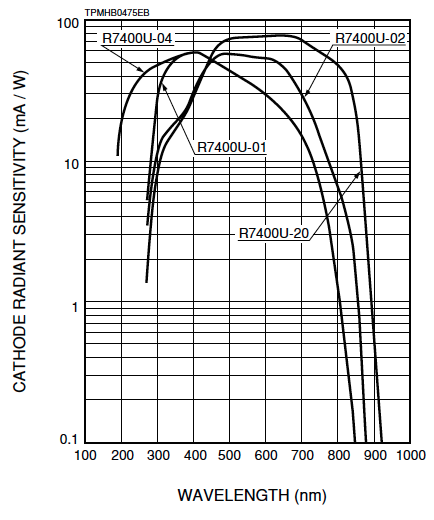
\includegraphics[width=0.85\textwidth]{appendices/pmtsensi}
\caption{Sensibilidad de respuesta del PMT. \emph{\scriptsize{Imagen adquirida de la hoja de especificaciones del PMT marca HAMAMATSU modelo R7400U-01.}}}\label{kk}
\end{figure}




 %es necesario introducir un factor de correci\'on.


%\footnote{Este factor de correcci\'on se obtiene de las curvas de respuesta del PMT contenidas el manual de dicho equipo} 


